\documentclass[fleqn]{jbook}
\usepackage{physpub}

\begin{document}

\begin{question}{専攻 問題2}{}

% Definition of local macros


\begin{center}
  \mbox{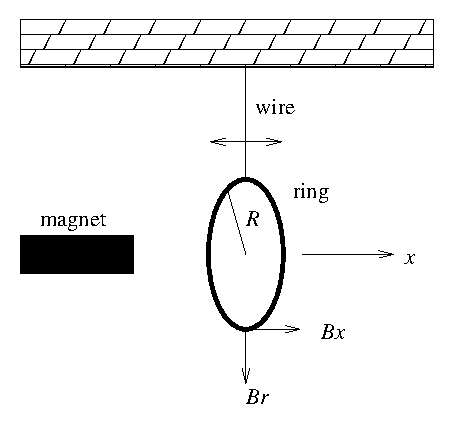
\includegraphics[clip]{1995phy2-1.eps}}
\end{center}

磁場中におかれた単振り子の一次元振動について考える。図に示すように、
振り子は導線を円形にしたリングと、それを吊す絶縁体のワイヤーから
できている。導線の太さはリングの半径$R$に比べて十分細い。静止状態で
のリングの中心軸を$x$軸にとり、リングの$x$座標の平衡位置からのずれを
$x(t)$とする。振り子の振幅は十分小さく、リングの中心軸は常に$x$軸に
一致しているとみなせるとする。磁場がないときのリングの運動方程式は
%
\begin{equation}
  m\left(\Deriver{^2 x}{t^2}+\omega_0^2 x\right) = f(t) \eqname{1}
\end{equation}
%
とあらわすことができる。ここで、$m$は振り子の質量、$\omega_0$は固有
角振動数。$f(t)$は外力である。図のように$x$軸に沿って細長い棒磁石が
置かれており、$x$軸に関して軸対称な磁場をつくっている。磁束密度の
リングの中心から半径方向の成分を$B_r$、$x$方向の成分を$B_x$とする。
リングの導線の位置での磁場に関して、$B_r$は振動の範囲以内では一様と
みなせるとする。このような磁場中に置かれたリングの振動について、
以下の問題に答えよ。ただし、{\bf 1}から{\bf 3}の問題においては、
リングのインダクタンスは無視できるものとする。



\begin{subquestions}
\SubQuestion
  まずリングの一周の抵抗値が$r$の場合を考える。リングを磁場中で振動
  させると、その運動は電磁誘導の作用により減衰する。このとき、最初に
  リングがもっていた運動エネルギーはどこに失われたかを述べよ。また、
  このエネルギー損失の割合を大きくするためには、抵抗値$r$が大きい方
  がよいか、小さい方がよいか、理由をつけて答えよ。

\SubQuestion
  \begin{subsubquestions}
  \SubSubQuestion
    運動にともない、リングに発生する誘導起電力$e$が
%
    \[ e = -2 \pi R B_r \Deriver{x}{t} \]
%
    となることを示せ。

  \SubSubQuestion
    磁場中でのリングの運動方程式を求めよ。

  \end{subsubquestions}

\SubQuestion
  次に、リングを静止させた状態で、$f(t)=p_0\delta(t)\quad$ ($\delta(t)$
  はDiracの$\delta$関数、$p_0$は定数)の外力を与えたときの $t\geq0$に
  おける振動を時間の関数として求め、その概略を図示せよ。

\SubQuestion
  \begin{subsubquestions}
  \SubSubQuestion
    抵抗値$r$がある程度小さくなると、リングの自己インダクタンス$L$
    が運動に効き始める。抵抗とインダクタンスの間にどのような関係が
    あるとき、インダクタンスによる効果が支配的になるかを答えよ。

  \SubSubQuestion
    この条件が成立する場合について、磁場中でのリングの運動方程式を
    求め、式\eqhref{1}で表されるような振動がどのような影響を受けるか
    を述べよ。
  \end{subsubquestions}
\end{subquestions}
\end{question}
\begin{answer}{専攻 問題2}{}

% Definition of local macros

\begin{subanswers}
\SubAnswer
  運動エネルギーは、リングの抵抗から発するジュール熱となって失われる。
  リングに発生する起電力が$V$のとき($V=-\Deriver{\Phi}{t}$より$V$は$r$に依らない)、ジュール熱が
  \[ VI = \frac{V^2}{r} \]
  であることから運動エネルギーの損失の割合は抵抗が小さい方が大きい。


\SubAnswer
  \begin{subsubanswers}
  \SubSubAnswer
    リングが磁場中を運動するとローレンツ力によりリングの周に電場が
    生じる。電場の強さ$E$を磁石側から見てリングの左周りを正として
    表すと
%
    \[ E = -\Deriver{x}{t} B_r \]
%
    となる。よってリング一周での電位差である $e$ は
%
    \[ e = 2 \pi R E = - 2 \pi R B_r \Deriver{x}{t} \]
%
    である。


  \SubSubAnswer
    リングに発生する誘導起電力によって流れる電流 $I$ は、
%
    \[ I = \frac{e}{r} = - \frac{2 \pi R B_r}{r} \Deriver{x}{t} \]
%
    磁場との相互作用によりリングは次の力 $f_I$ を受ける。
%
    \[f_I=I B_r 2 \pi R = -\frac{(2 \pi R B_r)^2}{r} \Deriver{x}{t} \]
%
    よって、リングの運動方程式は以下の通り。
%
    \[ m\left(\Deriver{^2 x}{t^2}+\omega_0^2 x\right)%
       = - \frac{ (2 \pi R B_r )^2 }{r} \Deriver{x}{t} + f(t) \]
%

  \end{subsubanswers}


\SubAnswer
  前問の結果で $\gamma\equiv(2\pi R B_r)^2/mr$ と書き改め
  撃力 $f(t)=p_0 \delta(t)$ を代入すると次の運動方程式を得る。
%
  \[ \Deriver{^2 x}{t^2} + \gamma \Deriver{x}{t} + \omega_0^2 x%
     = \frac{p_0}{m} \delta(t) \]
%
  この方程式を$[-\IDelta t,+\IDelta t]$の間で積分して$\IDelta t\to+0$の極限を
  とる。すなわち、
%
  \[ \lim_{\IDelta t\to +0} \Dint{-\IDelta t}{+\IDelta t}{\d{t}}\,\,\, \Bigl[ \Deriver{^2 x}{t^2}%
    + \gamma \Deriver{x}{t} + \omega_0^2 x \Bigr]%
    = \lim_{\IDelta t\to +0} \Dint{-\IDelta t}{+\IDelta t}{\d{t}}\,\,\,\frac{p_0}{m}\delta(t)\]
  \[ \lim_{\IDelta t\to +0}  \Biggl[ \Deriver{x}{t}\Bigm|_{-\IDelta t}^{+\IDelta t}%
    + \gamma x \Bigm|_{-\IDelta t}^{+\IDelta t}%
    + \frac{1}{2}\omega_0^2 x^2 \Bigm|_{-\IDelta t}^{+\IDelta t} \Biggr]%
    = \frac{p_0}{m} \]
%
  $x$の値は$t=0$において連続であるべきなので、この左辺第2項と第3項は
  $\IDelta t\to0$の極限で消える。第1項は残りこれはリングの速度が$t=0$
  で不連続であることを示す。すなわち$t=+0$での速度が得られる。
  $t=+0$では、撃力は既に働いていないので、$t>0$での運動方程式は次のように簡単化
  される。
%
  \[ \Deriver{^2 x}{t^2} + \gamma \Deriver{x}{t} + \omega_0^2 x = 0%
  \hspace{8mm} t>0 \hspace{8mm} x|_{+0}=0 \quad \Deriver{x}{t}\Bigm|_{+0} = \frac{p_0}{m} \]
%
  この線形の斉次微分方程式を解く。$x=e^{\lambda t}$の型の解を仮定して
  この方程式に代入すると次の結果を得る。
%
  \[ \lambda_{\pm}=\frac{-\gamma\pm\sqrt{\gamma^2-4\omega_0^2}}{2} \]
%
  $\gamma^2-4\omega_0^2\ge 0$ の場合には $\lambda_{\pm}$ は
  両者とも負の実数である。$x$の解は初期条件を考慮して次のようになる。
%
  \begin{eqnarray*}
  x &=& \frac{p_0}{m\sqrt{\gamma^2-4\omega_0^2}}%
        \bigl( e^{\lambda_{+}t}-e^{\lambda_{-}t} \bigr) \\
    &=& \frac{p_0}{m\sqrt{\gamma^2-4\omega_0^2}}%
        \left[ \exp{\left(\frac{-\gamma+\sqrt{\gamma^2-4\omega_0^2}}{2}t\right)}-\exp{\left(\frac{-\gamma-\sqrt{\gamma^2-4\omega_0^2}}{2}t\right)} \right]
  \end{eqnarray*}
%
  他方、$\gamma^2-4\omega_0^2<0$ の場合には $\lambda_{\pm}$ は
  両者とも複素数である。$x$の解は初期条件を考慮して次のようになる。
%
  \begin{eqnarray*}
  x &=& \frac{p_0}{m\sqrt{4\omega_0^2-\gamma^2}}%
        \exp{\left(-\frac{1}{2}\gamma t\right)}2\sin{\left(\frac{\sqrt{4\omega_0^2-\gamma^2}}{2}t\right)}
  \end{eqnarray*}
%
  この$x$の時間発展の様子は右下の図の様である。
%
\SubAnswer
  \begin{subsubanswers}
  \SubSubAnswer
  \parbox[t]{60mm}{
    自己インダクタンスの効果がある場合のリングを流れる電流$I$の
    満たすべき方程式は
%
    \[ 2\pi R B_r \Deriver{x}{t} - L\Deriver{I}{t} = rI \]
%
    であるが、$L$の項が比較的小さいと仮定して第0次近似で
%
    \[ 2\pi R B_r \Deriver{x}{t} = rI \]
%
  }\parbox[t]{95mm}{
  \begin{center}
     \mbox{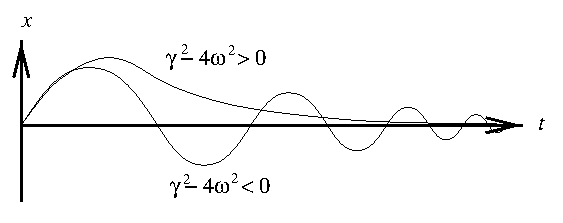
\includegraphics[clip]{1995phy2-2.eps}}
  \end{center}}\\
%
    を仮定し、この$I$を正確な方程式の$L$の項に代入する逐次近似法を
    採用する。したがって
%
    \[ I = \frac{2\pi R B_r}{r}\Deriver{x}{t} - L\frac{2\pi R B_r}{r^2}\Deriver{^2x}{t^2} \]
%
    となる。$I$の表式の右辺第2項はインダクタンスの影響の項である。
    これよりインダクタンスの効果が支配的となる条件は
%
    \[ \Bigm|\Deriver{x}{t}\Bigm| \ll \frac{L}{r}\Bigm|\Deriver{^2x}{t^2}\Bigm| \]
%
    である。この$x$の微分の量の大きさを見積もるために設問{\bf 3}
    で得られた式の $t \sim 0$ 付近での値を用いると、
%
    \[ \Deriver{x}{t} \sim  \frac{p_0}{m} \hspace{15mm}%
       \Deriver{^2 x}{t^2 } \sim - \frac{p_0}{m} \gamma \]
%
    これを代入して整理して、
%
    \[ r^2 \ll \frac{(2 \pi R B_r)^2 }{m} L \]
%
    この条件が満たされる時にインダクタンスによる効果が支配的となる。


  \SubSubAnswer
    インダクタンスによる効果が支配的な場合、運動方程式は下のよう
    になる。
%
    \[ m \left( \Deriver{^2 x}{t^2} + \omega_0^2 x \right)%
       = L \frac{(2 \pi R B_r)^2 }{r^2 } \Deriver{^2 x}{t^2 } + f(t) \]
%
すなわち、
    \[ ( m - \alpha )\left( \Deriver{^2 x}{t^2} + \frac{m}{m - \alpha } \omega_0^2 x \right) = f(t)%
       \hspace{10mm}%
       {\rm where}\quad \alpha = L \frac{(2 \pi R B_r)^2 }{r^2 } \ge 0 \]  
%
    つまり、リングの質量が減少して固有振動数が増加したと考えることができる。

  \end{subsubanswers}
\end{subanswers}
\end{answer}


\end{document}
